\subsection{The Quark-Gluon Plasma}
\label{sec:QGP}

The prior discussion of QCD involved hadrons in a vacuum at zero temperature; however, studying strong dynamics at nonzero (high) temperatures or baryon densities provides a novel environment for testing QCD.
This QCD environment is very rare in nature, being found only in two places~\cite{QGP:instantons}.
The first is in the interior of neutron stars, where the baryon density greatly exceeds normal nucleon densities.
The second is around $10^{-5}$ s after the Big Bang, when the temperature of the entire universe was very large, comparable to the nucleon rest mass.
Additionally, this high-temperature regime can be synthesized in a laboratory with collisions of relativistic heavy ions.

Models have long shown that nuclear matter is influenced by its thermodynamic environment.
The Bootstrap model by Hagedorn~\cite{QGP:Hagedorn}, before acceptance of the parton model, posits that the density of available hadronic states increases exponentially with the temperature of a system.
The result is that, at a given temperature $T_H$, the partition function for the hadronic states diverges, and any additional energy input into the system will create additional hadrons but will not increase the temperature.
The Bootstrap model estimated this temperature to be roughly $T_H = 160$ \MeV.

With the discovery of asymptotic freedom, it was found that the hadronic couplings become weak at high temperatures, leading to a state of matter where the degrees of freedom go from hadrons to quarks and gluons.
This transition is related to the restoration of chiral symmetry in QCD~\cite{QGP:Review}; in cold hadronic matter, the pions are the Goldstone bosons of a spontaneously broken chiral symmetry.
This state of nuclear matter, originally described in Reference~\cite{QGP:AsymFreeQuarks} as ``quark soup'', has become known as the Quark-Gluon Plasma (QGP).
This led to the reinterpretation of $T_H$ as a phase transition point, i.e., the critical temperature above which quarks are liberated from hadrons~\cite{QGP:TH}.

\subsubsection{Phase Diagram of Nuclear Matter}
\begin{figure}[H]
    \centering
    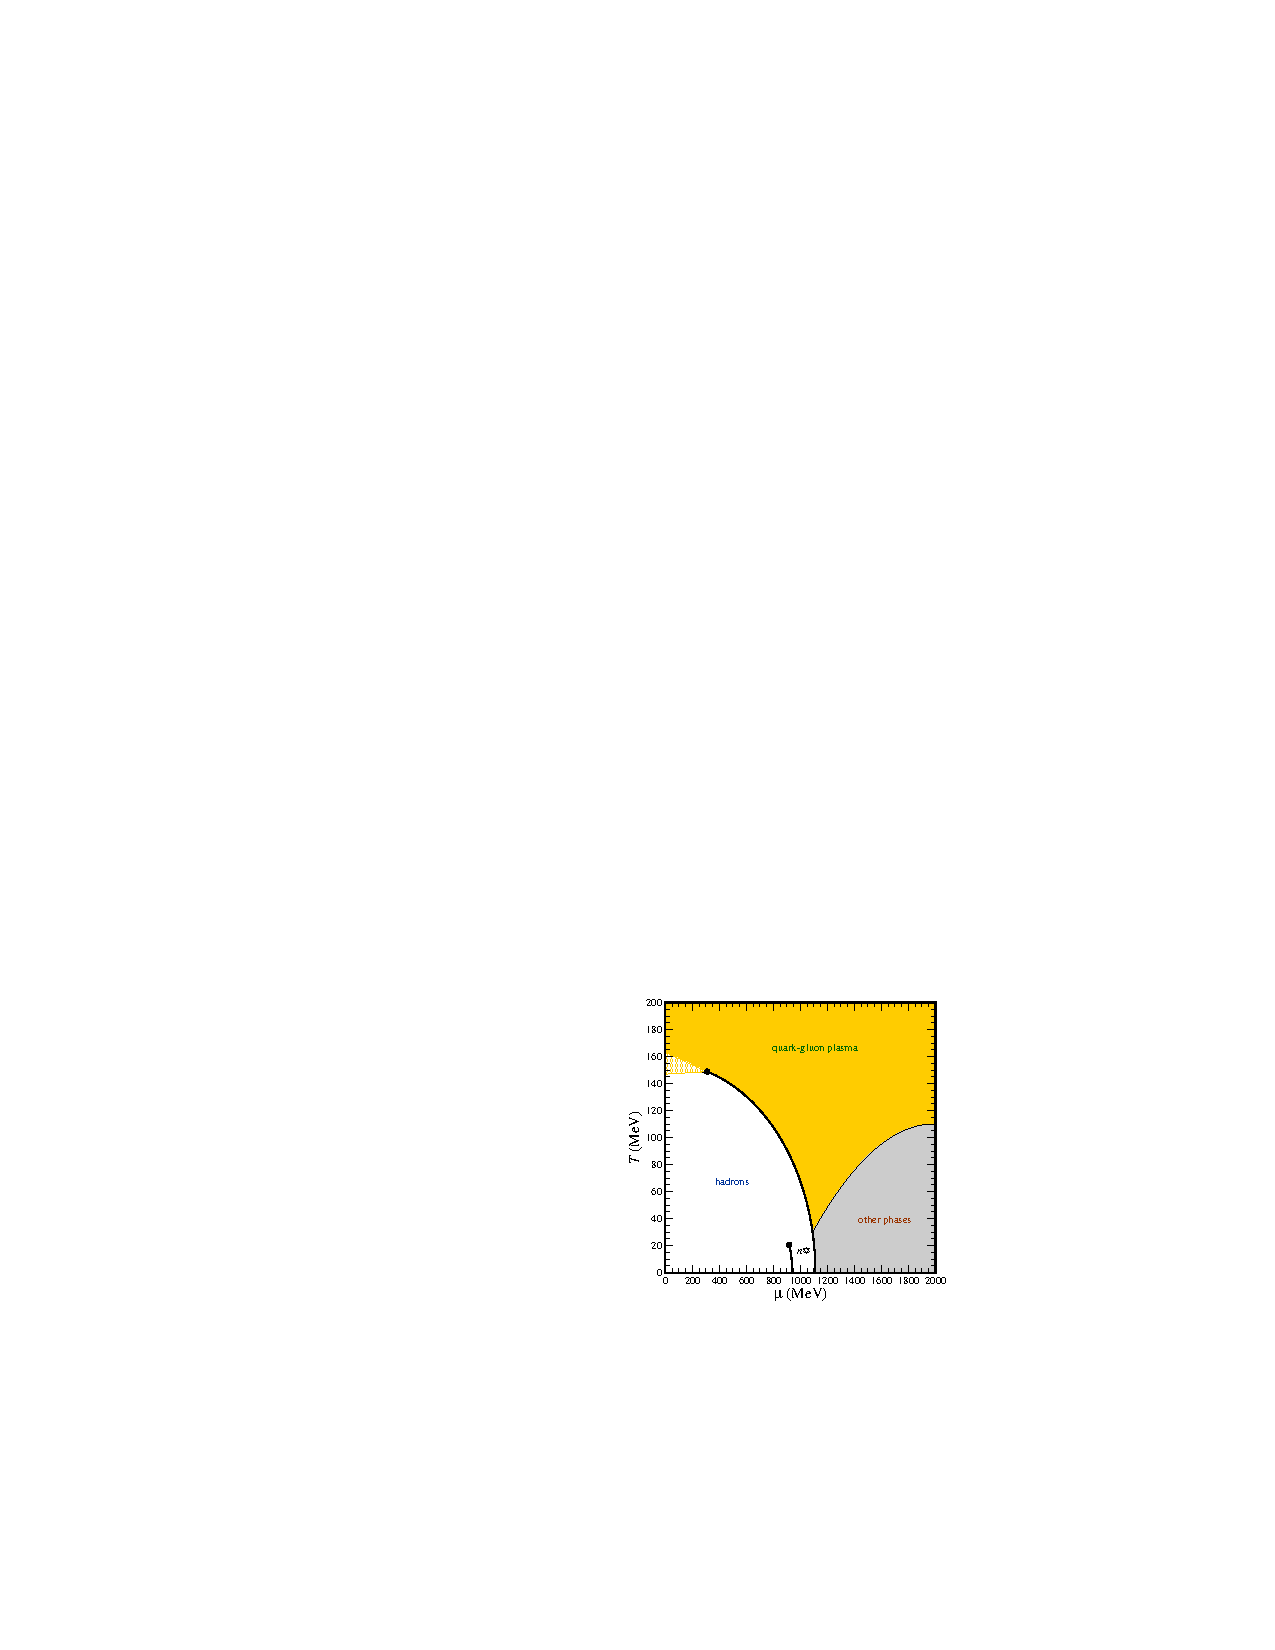
\includegraphics[
        width=0.8\linewidth,
        alt={Phase diagram of nuclear matter as a function of baryon chemical potential and temperature.}
    ]{chapters/background/sections/quark_gluon_plasma/figures/qgpphasediagram.pdf}
    \caption{Phase diagram of nuclear matter in the baryon chemical potential ($\mu$) and temperature ($T$) plane. Taken from Ref.~\cite{QGP:Lattice2}.}
    \label{fig:qgp_phase_diagram}
\end{figure}

The phase diagram for QCD matter is shown in Figure~\ref{fig:qgp_phase_diagram}.
The baryon chemical potential is related to the net baryon density.
At low baryon density, the crossover between the hadronic phase and the QGP is a smooth transition.
The nature of this transition is related to the nonzero quark masses.
As the phase diagram moves towards higher $\mu$, lattice calculations indicate that the transition may become a first-order phase transition~\cite{QGP:Lattice2}.
At very high baryon density, exotic states such as a color superconductor are postulated to exist, but this portion of the phase diagram is less well studied~\cite{QGP:superconductor}.
Heavy ion collisions at higher and higher energies probe the region of the QGP diagram at low-$\mu$ and high-$T$, because the ratio of baryon number to entropy scales inversely with collision energy.

\subsubsection{Timeline of an ion collision}
\begin{figure}[H]
    \centering
    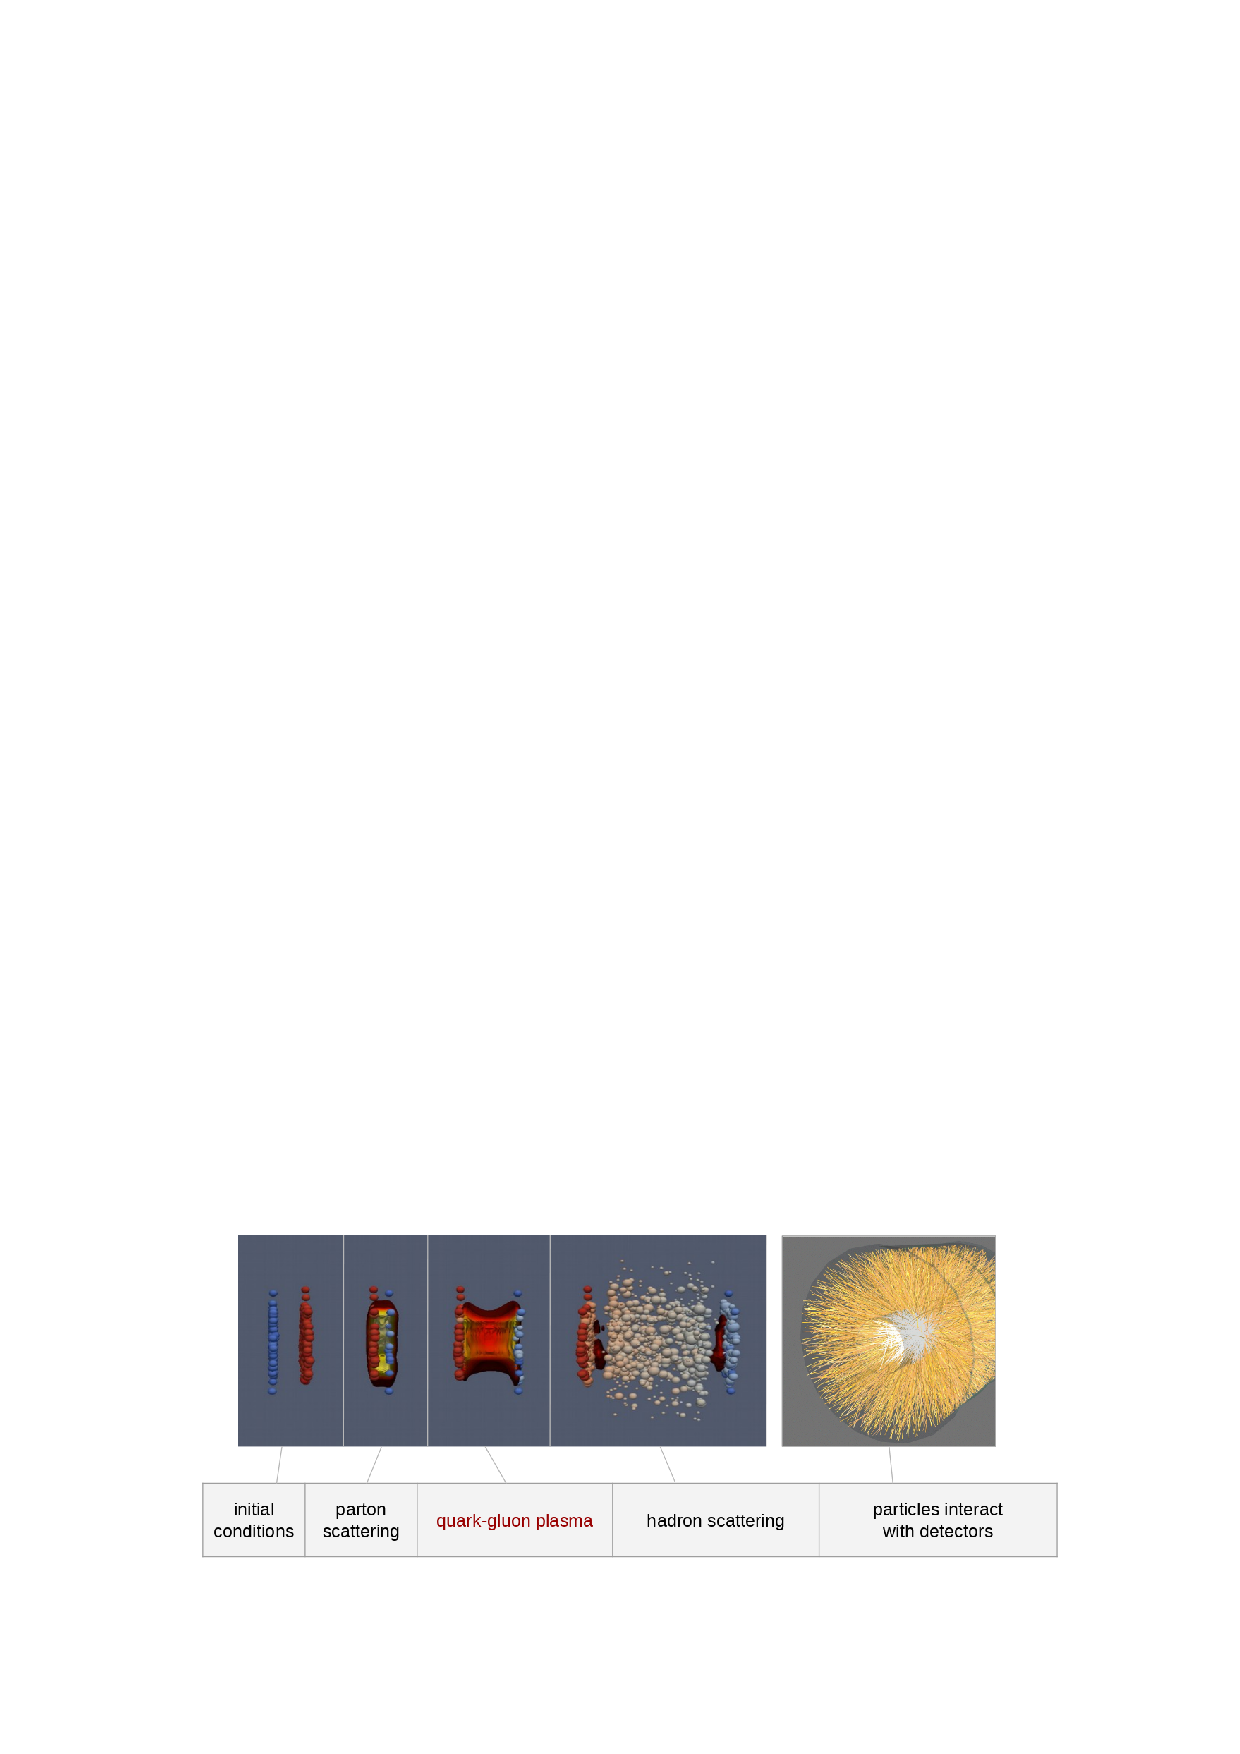
\includegraphics[
        width=0.9\linewidth,
        alt={Cartoon showing the successive stages of a relativistic heavy-ion collision, from the initial nuclei through the evolving quark-gluon plasma to final hadrons.}
    ]{chapters/background/sections/quark_gluon_plasma/figures/hicollisionstages.pdf}
    \caption{Cartoon illustrating the stages of a heavy-ion collision. Image from Reference~\cite{QGP:collisionTimeline} originally by H. Petersen and J. Bernhard, MADAI Collaboration.}
    \label{fig:heavy_ion_collision_stages}
\end{figure}

The QGP exists for only a short time during a heavy-ion collision. To study its properties, it is important to understand how the collision evolves into and out of the QGP state.
The different stages of an ion collision are described in Figure~\ref{fig:heavy_ion_collision_stages}.

\paragraph{Initial Conditions} The collision consists of two ions overlapping with some impact parameter $b$, which can be related to the centrality of the collision (as discussed in Section~\ref{sec:glauber}).
Centrality affects the transverse volume and shape of the later QGP medium: a central collision has a roughly circular overlap region, while a peripheral collision has a more lenticular overlap region.
The partonic content of the interacting nucleons is also modified by nPDFs, as discussed in Section~\ref{sec:nPDF}.

\paragraph{Pre-equilibrium/parton scattering}
As the nuclei cross each other at a time of 0 fm/$c$, most nucleon--nucleon collisions are of the low-$Q^2$ variety.
Nucleon--nucleon collisions also happen at a much higher $Q^2$, but they are a small fraction of the total $N_{\mathrm{coll}}$.
At $t>0$ fm/$c$, the two nuclei begin to separate at the speed of light, carrying most of the baryon density away from the collision point.
As the two receding nucleons are pulled apart, the \textit{glasma} state forms, which can be described as a ``color capacitor plate'' where longitudinal color field lines are formed between the two ions~\cite{QGP:Glasma}.
The Glasma is not yet an equilibrated QGP, but it is an early state dominated by strong longitudinal color fields that evolve and produce particles.

\paragraph{QGP formation} Over roughly the first $1$ fm/$c$ after the initial collision, the Glasma evolves into hot, dense matter that forms the QGP.
The system hydrodynamizes, meaning that viscous hydrodynamics becomes a useful macroscopic description.
The QGP behaves like a nearly perfect fluid, with a small shear-viscosity-to-entropy-density ratio, $\eta/s$~\cite{QGP:Review3}.
As time moves forward, the QGP expands hydrodynamically according to the pressure gradients in the system.

\paragraph{Hadronization and freezeout}
The QGP cools as it expands, with the temperature eventually falling below the crossover from QGP to the hadronic phase of matter.
During this phase, the unbound, interacting quarks and gluons start to hadronize.
At a temperature called the \textit{chemical freezeout temperature}, the partons have mostly become confined into hadrons, and no more inelastic interactions occur between them.
At this stage, the number of specific hadron types in the final state is fixed, although they may still elastically interact with each other.
At a later stage, kinetic freezeout occurs at the \textit{kinetic freezeout temperature}; at this point, the spacing between the final-state hadrons becomes so large that interactions are negligible.
At this stage, the momentum spectrum of the hadrons becomes fixed, and the final-state particles free-stream towards the detector, where they can be observed experimentally.

\subsubsection{Soft probes of the QGP}

Observables related to the low-momentum bulk particles produced in a heavy-ion collision can be sensitive tools for unveiling the nature, size, and evolution of the QGP.
Specifically, the azimuthally differential yields of final-state particles, typically referred to as \textit{flow}, are related to the transverse extent of the medium.
These yields can be written as a Fourier expansion of the $\frac{\mathrm{d}N}{\mathrm{d}\phi}$ distribution:
\begin{equation}
    \label{eq:flow_fourier}
    \frac{\mathrm{d}N}{\mathrm{d}\phi}
    \propto 1 + 2\sum_{n=1}^{\infty}
    v_n\cos\left(n(\phi-\Psi_n)\right)
\end{equation}
where $N$ is the number of final-state hadrons, $\phi$ is the azimuthal angle, $\Psi_n$ is the ``so-called'' event-plane angle, and $v_n$ are the $n$th-order flow coefficients.
The event-plane angle is an estimate of the direction of maximal particle emission for a specific harmonic $n$.
For $n=2$, the event-plane angle roughly tracks the azimuthal angle of the impact-parameter vector $\vec{b}$.
The sum in Equation~\ref{eq:flow_fourier} is over all particles in a given event, though typically only charged particles are available experimentally.
The flow coefficients observed experimentally are averages of the coefficients extracted event by event.

For heavy-ion events with non-negligible $b$, the fireball formed will be less circular (left side of Figure~\ref{fig:qgp_flow}) and more lenticular (right side of Figure~\ref{fig:qgp_flow}).
The pressure of the QGP fluid is at a maximum in the center of the medium and is zero in the vacuum outside it.
Therefore, pressure gradients will form across the medium, which will be counteracted by the shear viscosity of the medium.
This gradient will have a larger value across the shorter axis of the medium than the longer axis, inducing a more rapid hydrodynamic expansion along that direction.
After hadronization and freezeout, the result of this anisotropic expansion, called elliptic flow, is encoded in the $v_2$ flow coefficient of Equation~\ref{eq:flow_fourier}.
Measurements of elliptic flow provide important input into calculations of the shear viscosity of the medium~\cite{QGP:Review3}.
In fact, early RHIC data seem to favor a very low shear viscosity of the QGP fluid ($\eta / s \approx 0.1$)~\cite{QGP:RHICetas}, earning the QGP the name ``the most perfect fluid''.
Figure~\ref{fig:atlas_vn} displays a measurement of $v_2$ (among other coefficients) as a function of both charged-particle \PT\ and event centrality.
For very central events (small $b$), the medium formed is roughly circular, and therefore there is little azimuthal anisotropy in the pressure gradients, leading to smaller elliptic flow.
Compare that with more peripheral selections (higher $b$), where the fireball will take on a more lenticular shape, which then leads to a higher $v_2$.

\begin{figure}[H]
    \centering
    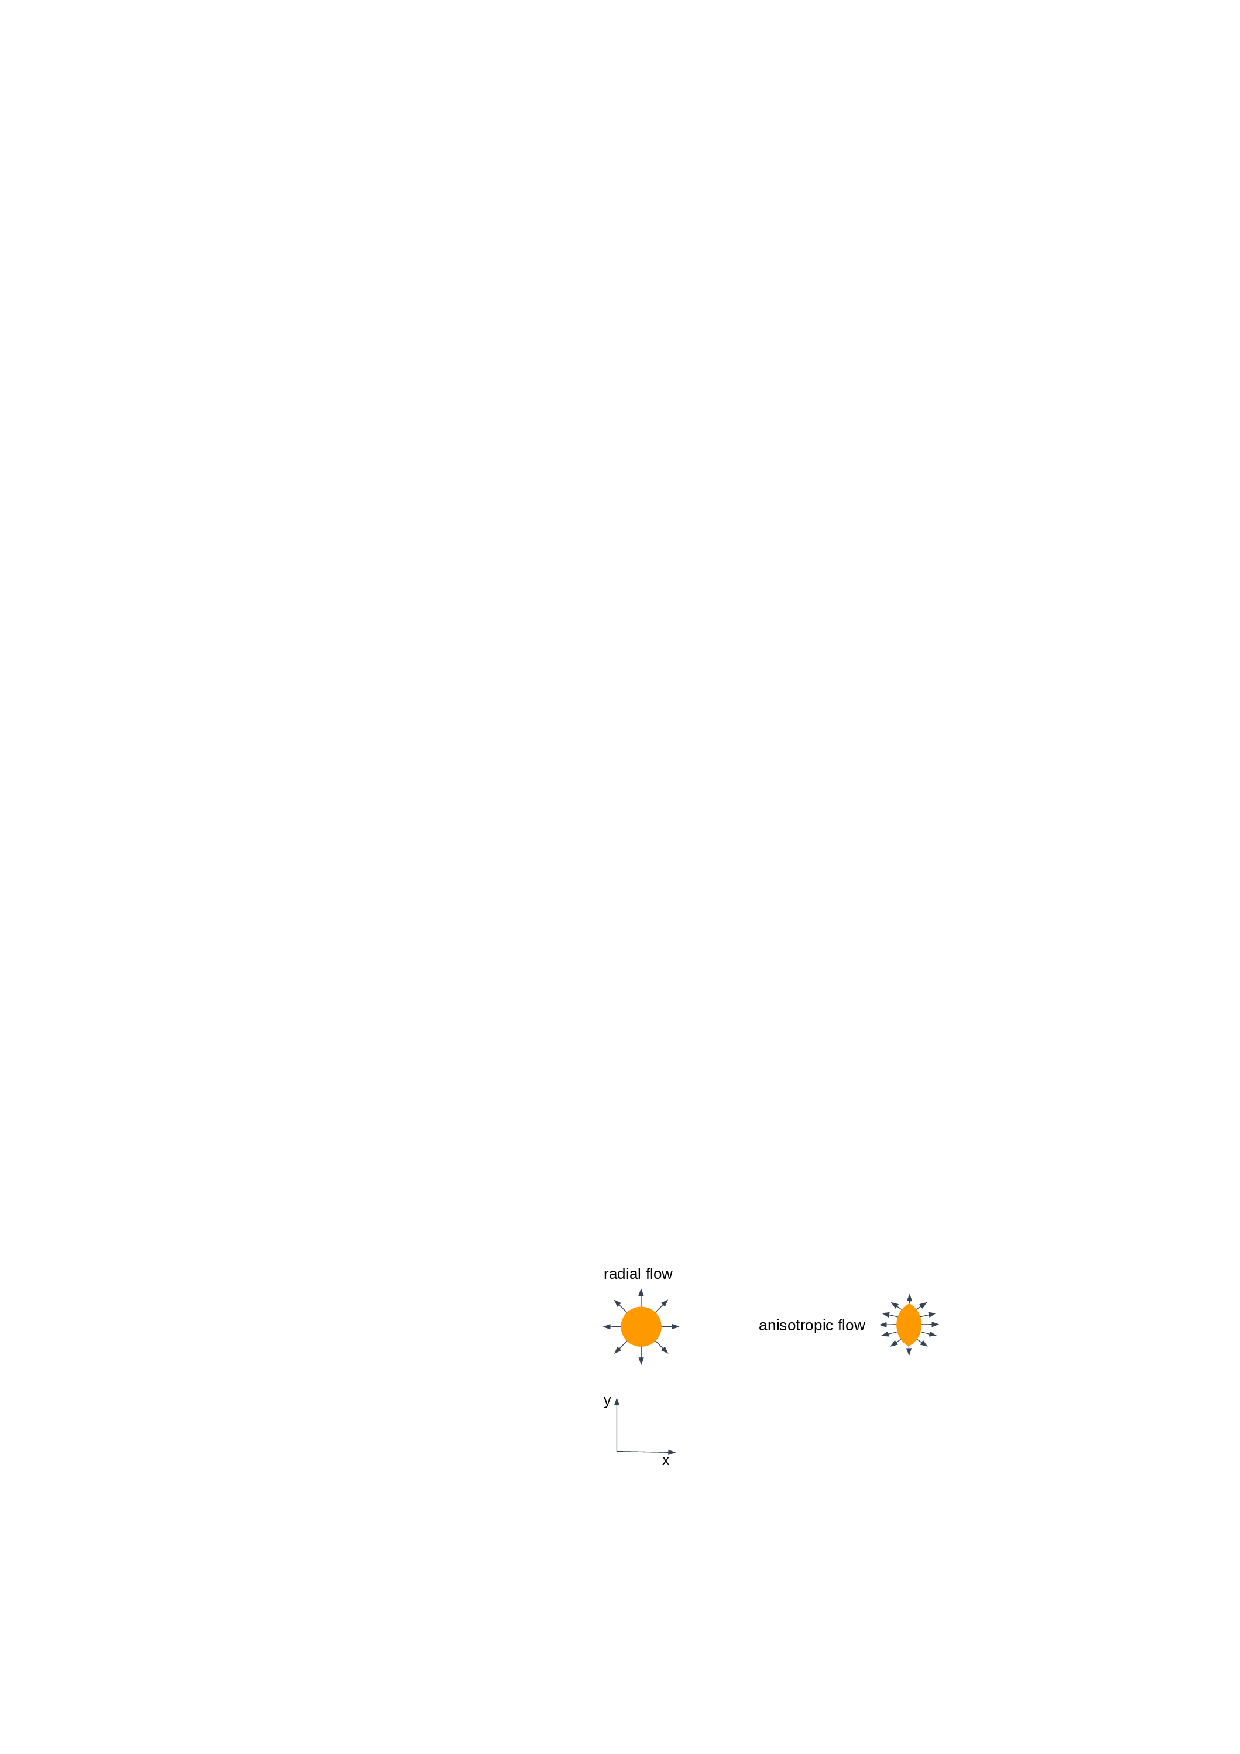
\includegraphics[
        width=0.8\linewidth,
        alt={Diagram illustrating the directionality of particle flow in a heavy-ion collision.}
    ]{chapters/background/sections/quark_gluon_plasma/figures/flowdiagram.pdf}
    \caption{\textcolor{red}{Schematic illustration of particle flow in a heavy-ion collision. Taken from Ref.~\cite{QGP:collisionTimeline}.}}
    \label{fig:qgp_flow}
\end{figure}

The zeroth-order flow coefficient, called radial flow, is not included in the forier decomposition of Equation~\ref{eq:flow_fourier} because it a represnts the collective isotropic expansion and does not vary with $\phi$.
The bulk viscosity of the QGP counteracts this radial acceleration; therefore, measurements of $v_0$ can help constrain this quantity~\cite{QGP:Review3}.
The left side of Figure~\ref{fig:qgp_flow} shows the isotropic expansion of the (orange) medium leading to radial flow.
The ATLAS experiment recently measured radial flow directly~\cite{HION-2024-06} in collisions with very small $b$, i.e., very central collisions.
Anisotropy in the $\frac{\mathrm{d}N}{\mathrm{d}\phi}$ distribution can result from either the geometry or fluctuations in the initial state.

\begin{figure}[H]
    \centering
    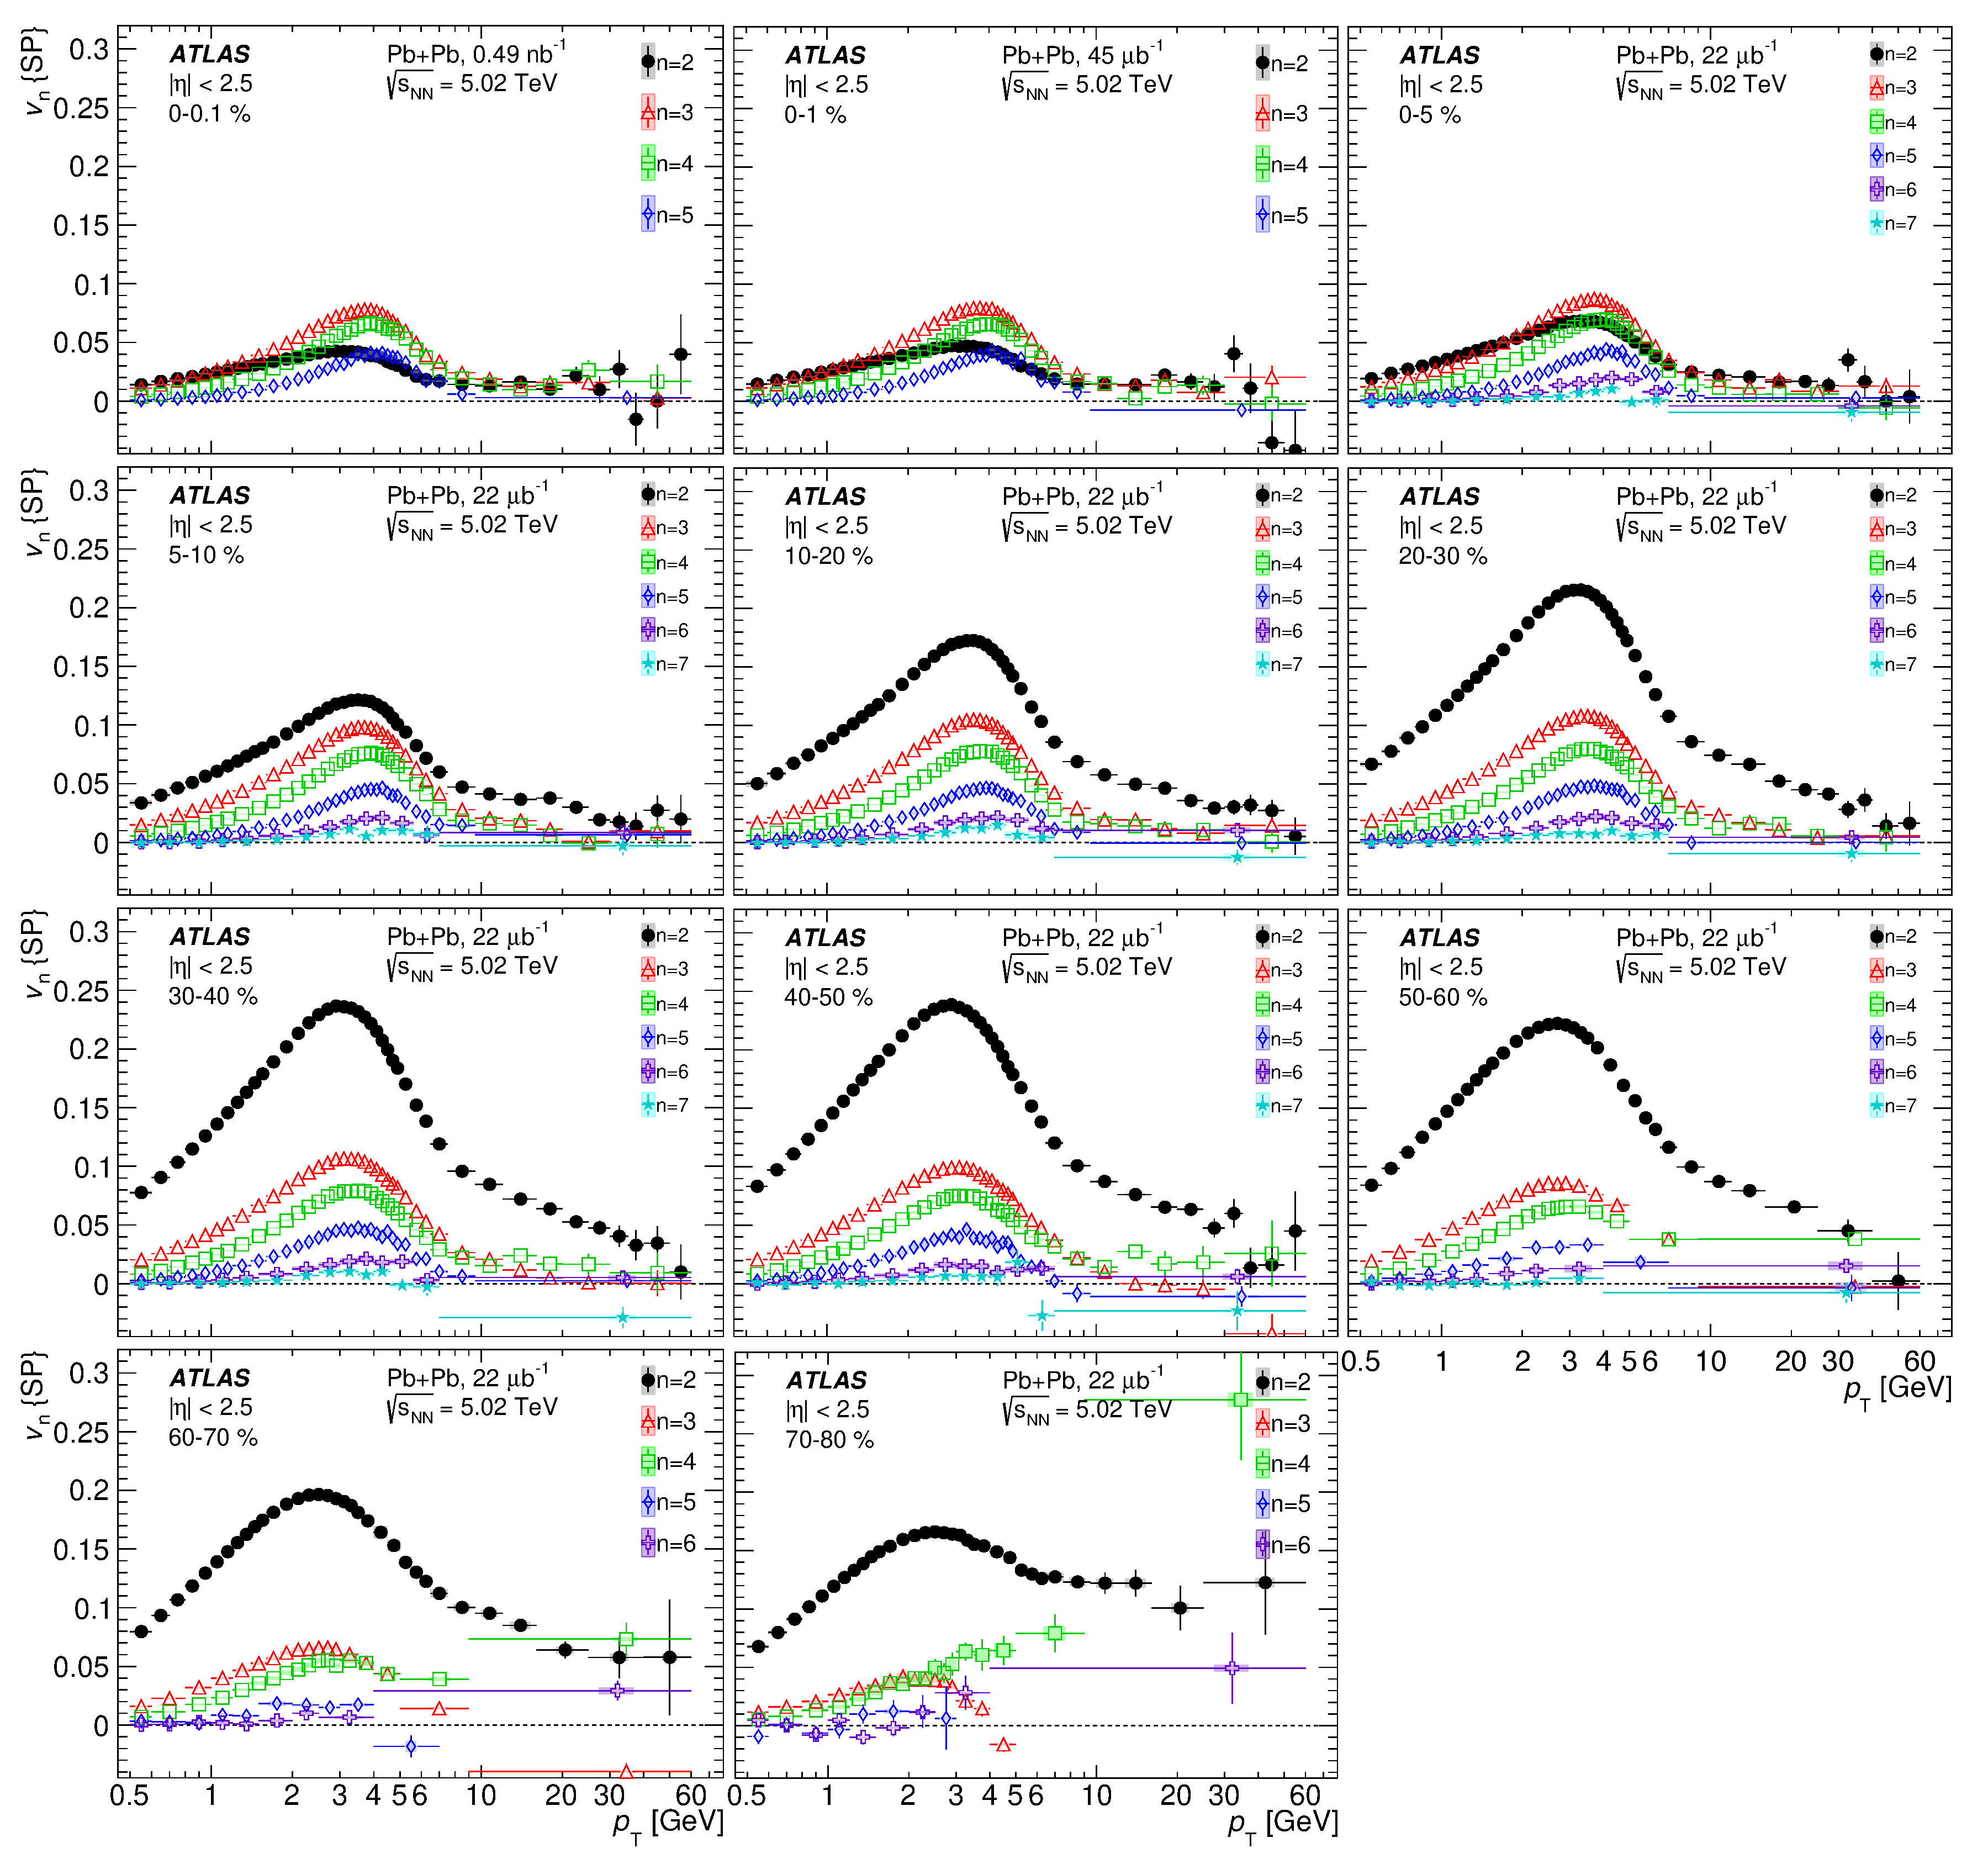
\includegraphics[
        width=0.75\linewidth,
        alt={ATLAS measurements of flow coefficients v two through v seven versus transverse momentum in eleven centrality intervals for charged particles within absolute pseudorapidity less than 2.5.}
    ]{chapters/background/sections/quark_gluon_plasma/figures/v_n_atlas.pdf}
    \caption{The $v_n$ obtained as a function of transverse momentum $p_T$ in 11 centrality intervals, from the most central at the top left panel to the most peripheral at the bottom right panel. Taken from Ref.~\cite{HION-2016-06}.}
    \label{fig:atlas_vn}
\end{figure}

Another source of transverse anisotropy in the QGP comes from fluctuations in the initial state.
If the optical Glauber approximation of smooth nuclear densities were correct, then all odd $v_n$ coefficients should vanish.
However, due to event-by-event fluctuations in the nucleon positions, these odd harmonics end up being non-zero.
The $v_3$ is termed triangular flow, and it extracts triangular structures inside the QGP fireball.
From Figure~\ref{fig:atlas_vn}, one can note that central collisions have azimuthal particle production dominated by fluctuations in the initial state because $v_{3,4}> v_2$ for many bins of \PT.
Experimentally, measuring flow signals can be complicated by the presence of high-$Q^2$ processes. For example, a dijet will produce some azimuthal anisotropy that does not come from the QGP.
Methods for subtracting such ``non-flow'' contributions are used to circumvent this problem.

Other bulk observables, such as the charged-particle pseudorapidity density, $\mathrm{d}N_{\mathrm{ch}}/\mathrm{d}\eta$, and transverse-momentum spectrum, $\mathrm{d}N_{\mathrm{ch}}/\mathrm{d}p_{\mathrm{T}}$, can also be used to infer properties of the medium.
The pseudorapidity density constrains the produced-particle multiplicity and, in turn, the medium's entropy production and initial density.
The low-$p_{\mathrm{T}}$ shape of the spectrum and the mean transverse momentum, $\langle p_{\mathrm{T}}\rangle$, are sensitive to the medium's expansion and radial flow.
These observables are interpreted together with models of the initial conditions and particle production.

\subsubsection{Jet quenching and hard probes of the QGP}

Jets are produced in the very early times of the heavy ion collision and as such they ``see'' the full lifecycle of the QGP. 


{\color{red}
    \begin{itemize}
        \item Explain how hard scatterings produce high-momentum partons that traverse the QGP and lose energy through medium-induced radiation and interactions.
        \item Introduce nuclear modification factors and reconstructed-jet observables as measures of suppression and energy redistribution.
        \item Describe dijet and photon/Z--jet momentum imbalance as tools for relating energy loss to the initial parton kinematics.
        \item Discuss dependence on parton energy, path length, and medium density, and the role of the transport coefficient $\hat{q}$.
        \item Explain how proton--nucleus and other reference measurements help distinguish QGP effects from initial-state and cold-nuclear-matter effects.
    \end{itemize}
}

\subsubsection{QGP in small systems}
\label{sec:qgp_small}
{\color{red}
    \begin{itemize}
        \item Define small collision systems, such as proton--proton and proton--nucleus collisions, and explain why QGP formation there was initially unexpected.
        \item Summarize collective signatures in small systems, including long-range correlations and flow-like patterns, and compare them with heavy-ion results.
        \item Discuss possible origins of these signatures, including hydrodynamic response, initial-state correlations, and the role of event activity.
        \item Review the evidence and open questions concerning jet quenching and other final-state effects in small systems.
        \item Motivate using small systems as a test of the minimum conditions for QGP-like behavior and as a baseline for nuclear-collision measurements.
    \end{itemize}
}
